\documentclass{article}
\title{Absence versus Presence of Dissipative Quantum Phase Transition in Josephson Junctions}
\usepackage{physics}
\usepackage{mathrsfs}
\usepackage{amssymb}
\usepackage{graphicx}
\begin{document}
\section{Abstract to Introduction}
Dissipative quantum phase transition, always occurs Josephson Junction system, when $R_Q=h/4e^2$.\\
 \\

\begin{figure}[!h]
    \centerline{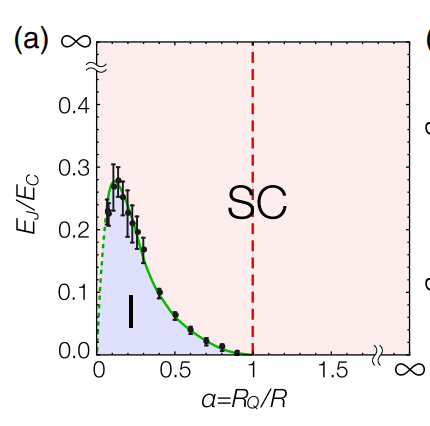
\includegraphics[width=\columnwidth]{Phy129087001_1.png}}
    \caption{Figure 1-(a) in given paper, Result of functional renormalization group (FRG) and numerical renormalization group (NRG)}
    \label{figure_1} 
\end{figure}
$E_C=(2e)^2/2C_J$ : Charging energy with the capacitance $C_J$\\
$\quad E_J$ : Josephson coupling\\
 \\ 
$\quad \alpha = R_Q=h/4e^2$ : different dissipation strengths $\alpha$. Transition occurs $\alpha < 1$.\\
\begin{table}[]
    \begin{tabular}{cc}
    \hline
    \multicolumn{1}{|c|}{$E_J/E_C << 1$}     & \multicolumn{1}{c|}{$E_J/E_C >> 1$}  \\ \hline
    \multicolumn{1}{|c|}{deep charge regime} & \multicolumn{1}{c|}{transmon regime} \\ \hline
    \multicolumn{1}{|c|}{?} & \multicolumn{1}{|c|}{Strong corrugation regime}       \\ \hline
    \end{tabular}
    \end{table}
If $R_Q/R(\propto \alpha) $ is decreased, results indicate the \textbf{reentrant transition}.\\
\textbf{Dangerously irrelevant} : $\nu \propto 1/E_C$ , Capacitance term , it can turn into relevant at low-energy scales due to nonperturbative renormalization.\\
$\rightarrow$ The reason that previous existed arguments missed.
\section{Discussion}
$\nu$ (Dangerously irrelevant term)  : Safely neglected can one establish the duality between the weak and strong corrugation regimes.\\
 \\ 
$E_J/E_C \gg 1$ : RSJ Hamiltonian ~ tight-binding model of phase localized states ($\phi=2\pi \mathbb{Z}$)\\
$\rightarrow$ Exhibits the transition at $\alpha_c = 1$,\\
$E_J/E_C \ll 1$ : both tight-binding and duality argument are expected to be valid.\\
$\rightarrow$ results from given paper are consistent with the previous results predicting the transition at $\alpha_c = 1$ for any $E_J/E_C$.\\
 \\
\textit{Experimentally test for predictions} : lowest transmission-line frequency $\omega_{min} = \pi v /L$.\\
\textit{Pre-requirements} : renormalize to a sufficiently low-energy scale to attain small $\langle \cos (\phi) \rangle$ close to a fixed-point value;\\
\textit{Parameters} : $\alpha =0.3\quad,\quad E_J/E_C = 0.04 \quad ,\quad \hbar \omega_{min}, k_B T \lesssim 0.01E_C \quad ,$ to attain $\langle \cos (\phi) \rangle \lesssim 10^{-2}$.
\\
 \\
These setup realized through the galvanic coupling of JJ to a high-impedance long transmission line.

\end{document}